\documentclass[a4paper,12pt]{article}

\usepackage[utf8]{inputenc}
\usepackage[T1]{fontenc}
\usepackage{a4}
\usepackage{lipsum}
\usepackage{graphicx}
\usepackage{float}
\usepackage{listings}
\usepackage{color}
\usepackage{hyperref}
\usepackage{cite}
\usepackage{textgreek}
\usepackage{amsfonts}
\usepackage{amsmath}

\usepackage[margin=1in]{geometry}

\definecolor{dkgreen}{rgb}{0,0.6,0}
\definecolor{gray}{rgb}{0.5,0.5,0.5}
\definecolor{mauve}{rgb}{0.58,0,0.82}

\lstset{frame=tb,
  language=matlab,
  aboveskip=5mm,
  belowskip=5mm,
  showstringspaces=false,
  columns=flexible,
  basicstyle={\small\ttfamily},
  numberstyle=\tiny\color{gray},
  keywordstyle=\color{blue},
  commentstyle=\color{dkgreen},
  stringstyle=\color{mauve},
  breaklines=true,
  breakatwhitespace=true,
  tabsize=2
}

\title{
  {\Huge \bf Power Systems Lab}\\
  \vspace{0.25in}

  {\bf Experiment 4}\\
  Laboratory Report
  \vspace{1in}
}
\author{
  \bf Syed Alisamar Husain, 17BEE012\\
  B.Tech Electrical Engg, 8th Semester
}

\begin{document}
  \begin{titlepage}
    \maketitle
    \vspace*{\fill}
    \begin{center}
      {\bfseries Department of Electrical Engineering} \\
      Jamia Millia Islamia, New Delhi
    \end{center}
    \thispagestyle{empty}
  \end{titlepage}
  
  \newpage
  \begin{center}
    \huge Experiment 4
    \vspace{0.5in}
  \end{center}

  \section{Objective}
  To write a MATLAB program to determine line currents to a Y-connected load
  by mesh analysis and by using symmetrical components.

  {\bf Let the given problem be as follows:}
  \begin{center}
    \itshape
    A balanced three phase voltage is applied to a Y-connected load with ungrounded 
    neutral. The three phase load consists of three mutually-coupled reactances.
  \end{center}
  \begin{enumerate}
    \itshape
    \item Determine the line currents by mesh analysis.    
    \item Determine the line currents by using symmetrical components.
  \end{enumerate}

  \section{Theoretical Background}
  Shown below is a 3-phase supply connected to a Y-connected load.
  \begin{figure}[H]
    \centering
    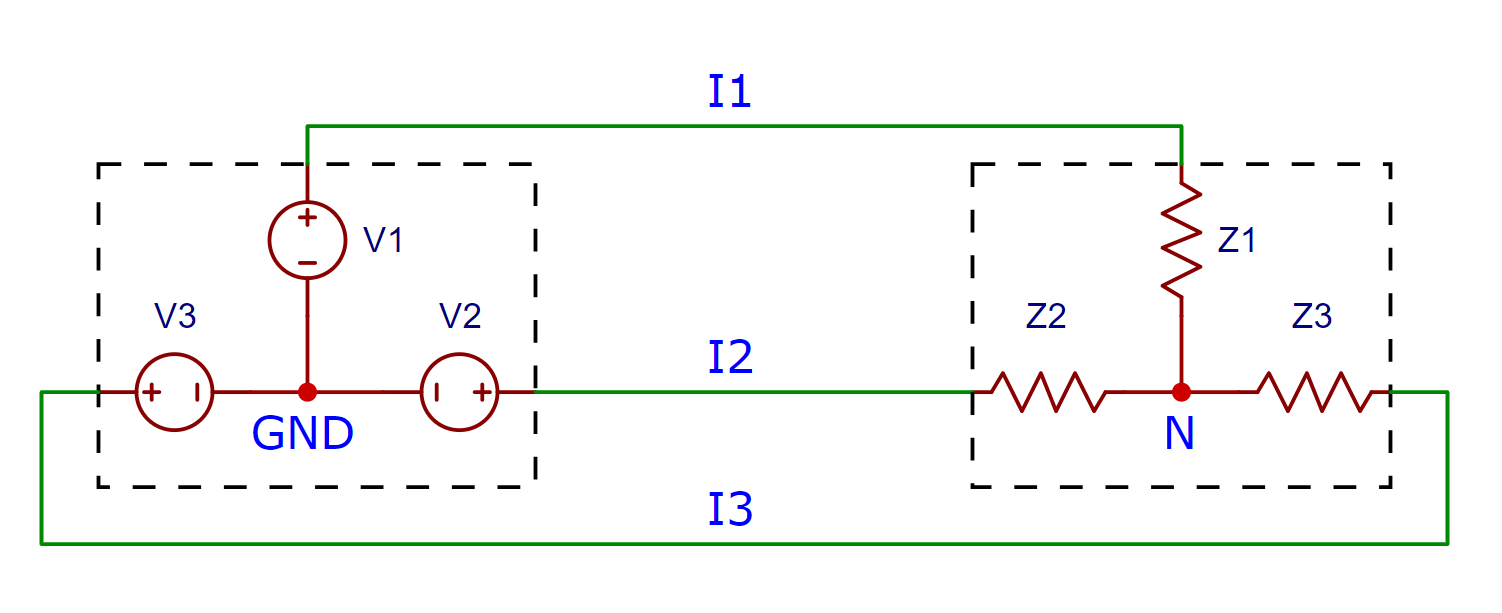
\includegraphics[width=5in]{img/y-load.png}
    \caption{Y-connected load with ungrounded neutral.}
    \label{yload}
  \end{figure}

    \pagebreak
    \subsection{Sequence Components}
    A set of three balanced voltages (phasors) $V_a, V_b, V_c$ is charactertzed by equal
    magnitudes and interphase differences of $120\deg$. The set is said to have a phase
    sequence $abc$ (positive sequence) if $V_b$ lags $V_a$ by $120\deg$ and $V_c$ lags 
    $V_b$ by $120\deg$.

    The three phasors can then be expressed in terms of the reference phasor $V_a$ as
    \begin{center}
      $V_a$ = $V_a$\\
      $V_b$ = $\alpha^2 V_a$\\
      $V_c$ = $\alpha V_a$\\
    \end{center}
    where the complex number operator $\alpha$ is defined as $\alpha = e^{j 120\deg}$.
    The same applies to voltages or currents.
    
    If the phase sequence is $acb$ (negative sequence), then
    \begin{center}
      $V_a$ = $V_a$\\
      $V_b$ = $\alpha V_a$\\
      $V_c$ = $\alpha^2 V_a$\\
    \end{center}

    Thus a set of balanced phasors is fully characterized by its reference phasor
    (say $V_a$) and its phase sequence (positive or negative).

    Consider now a set of three voltages (phasors) $V_a, V_b, V_c$ which in general may
    be unbalanced. According to {\bf Fortesque's theorem} the {\it three phasors can be
    described as the sum of positive, negative and zero sequence phasors}.

    \begin{center}
      $V_a = V_a^1 + V_a^2 + V_a^0$\\
      $V_b = V_b^1 + V_b^2 + V_b^0$\\
      $V_c = V_c^1 + V_c^2 + V_c^0$
    \end{center}

    The three phasor sequences (positive, negative and zero) are called the
    {\bf symmetrical components} of the original phasors. These equations 
    can be expressed in the matrix form
    
    \begin{center}
      \begin{math}
        \begin{bmatrix}
          V_a \\ V_b \\ V_c
        \end{bmatrix}
        =
        \begin{bmatrix}
          1 & 1        & 1 \\
          1 & \alpha^2 & \alpha \\
          1 & \alpha   & \alpha^2
        \end{bmatrix}
        \begin{bmatrix}
          V^0_a \\ V^1_b \\ V^2_c
        \end{bmatrix}
      \end{math}
    \end{center}

    \begin{center}
      $ \bf V_p = A V_s $\\
    \end{center}

    To find the sequence components, we can invert the equation
    \begin{center}
      $ \bf V_s = A^{-1} V_p $
    \end{center}

    \begin{center}
      where
      \begin{math}
        {\bf A^{-1}} =
        \dfrac{1}{3}
        \begin{bmatrix}
          1 & \alpha   & \alpha^2 \\
          1 & \alpha^2 & \alpha \\
          1 & 1        & 1
        \end{bmatrix}
      \end{math}
    \end{center}

  \pagebreak
  \section{Implementation}
  \begin{lstlisting}
    
  \end{lstlisting}

  \section{Observations}
  \begin{figure}[H]
    \centering
    % 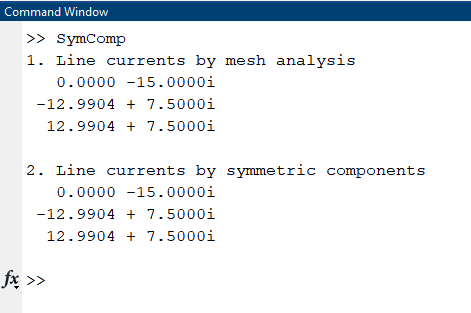
\includegraphics{img/run.png}
    \caption{Result in MATLAB}
    \label{result}
  \end{figure}
  The result of the above program with the given parameters 
  is shown in figure \ref{result}.

  \section{Result}

\end{document}